% ----------------------------------------------------------------------- %
% Arquivo: 04-Resultados.tex
% ----------------------------------------------------------------------- %
\chapter{Treinamento da Rede Neural para Detecção e localização de Defeitos em Placas de Circuito Impresso} \label{cap:treinamento}
%Falta escrever essa parte.
Nesse capítulo serão discutidas a escolha e as etapas de preparação do \textit{dataset} para o treinamento, detalhes de configurações da rede neural utilizada e os resultados obtidos.

\section{Seleção da Rede Neural e do \textit{Framework} para o Treinamento} \label{cap:treinamento-rn}

Defeitos em placas de circuito impresso ocupam pequenas regiões da PCI, de forma que a proporção entre a área do objeto a ser detectado e a imagem inteira é muito pequena. Sendo assim, a escolha da rede neural deve considerar um bom desempenho para detecção de pequenos objetos. Segundo \citeonline{ref:Redmon-Farhadi}, a partir da versão três, a YOLO apresentou uma melhor performance para esse tipo de detecção, sendo recomendada para essa aplicação por \citeonline{ref:Valenti-et-al}, quando o tempo de treinamento não é tão relevante. Já a versão quatro da YOLO apresenta melhor desempenho para o treinamento em GPUs quando comparada a sua versão anterior.

Sendo assim, a rede neural escolhida para o treinamento da detecção de defeitos em PCIs foi a YOLO em sua quarta versão, proposta por \citeonline{ref:Bochkovskiy-Wang-Liao} em conjunto com \textit{framework} Darknet, que possui funções de cálculo das métricas de avaliação, desenho das caixas delimitadoras, entre outras.

\section{Seleção do Conjunto de Dados} \label{cap:treinamento-dataset}

Para a detecção e classificação de objetos, o conjunto de dados escolhido deve incluir além das imagens, a localização e classificação dos objetos de interesse.
O \textit{Dataset} escolhido para a detecção e localização de defeitos em PCIs é o \textit{HRIPCB: a challenging dataset for PCB defects detection and classification}, proposto por \citeonline{ref:Huang-et-al}.

As imagens das placas são capturadas por uma câmera do tipo industrial com dezesseis megapixel de resolução equipada com um sensor C-MOS \cite{ref:Huang-et-al}. Após a captura e ajustes, seis tipos de defeitos são adicionados manualmente em um \textit{software} de edição de imagens, onde cada imagem contém de dois a seis defeitos da mesma categoria em diferentes lugares da placa \cite{ref:Huang-et-al}. A distribuição dos defeitos está na \autoref{tab:treinamento-dataset}.

\begin{table}[!h]
\begin{center}
\caption{Distribuição dos defeitos no conjunto de dados HRIPCB.}
\label{tab:treinamento-dataset}
\begin{tabular}{ccc}
\toprule
\textbf{Tipo do Defeito} & \textbf{Número de Imagens} & \textbf{Quantidade Total de Defeitos} \\
\midrule \midrule
Falta de Estanho    & 115   & 497 \\
Falta de Cobre      & 115   & 492 \\
Circuito Aberto     & 116   & 482 \\
Curto-Circuito      & 116   & 491 \\
Excesso de Cobre    & 115   & 488 \\
Trilha Desconectada & 116   & 503 \\
\bottomrule
\end{tabular}
\indentedfont[0.96\textwidth]{\citeonline{ref:Huang-et-al}}
\end{center}
\end{table}

Para cada uma das imagens, existe um arquivo com extensão \textit{.xml} que mapeia as informações das caixas delimitadoras de cada defeito. Um exemplo desse arquivo está no \autoref{apendice:hripcb-xml}.
As anotações do HRIPCB não estão normalizadas e e são mapeadas em coordenadas cartesianas em pixeis $x_{min}$, $x_{max}$, que variam entre zero e a largura da imagem e $y_{min}$, $y_{max}$, que variam entre zero e a altura da imagem, conforme a \autoref{fig:resultados-hripcb-notacao}.

\begin{figure}[h!] %H
  \centering
  \caption{Anotações das caixas delimitadoras do \textit{dataset} HRIPCB.}
  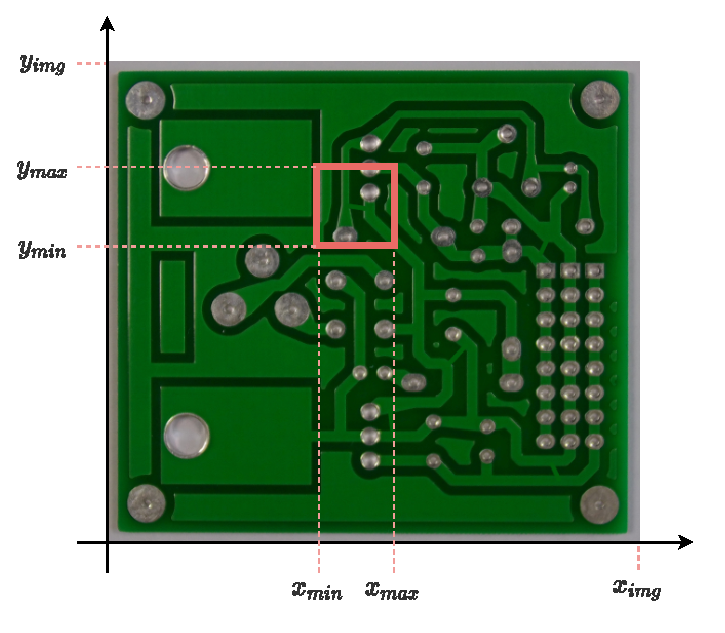
\includegraphics[scale=1]{img/img-resultados-hripcb-notacao.pdf}
  \label{fig:resultados-hripcb-notacao}
  \indentedfont[15.2cm]{Adaptado de \citeonline{ref:Huang-et-al}}
\end{figure}


A estrutura de arquivos do \textit{dataset} está na \autoref{fig:resultados-hripcb-estrutura}. Os arquivos dentro da pasta \textit{rotation} não foram utilizados já que não possuem as delimitações dos defeitos em arquivos de anotação.

\begin{figure}[h!] %H
  \centering
  \caption{Estrutura de arquivos do \textit{dataset} HRIPCB.}
  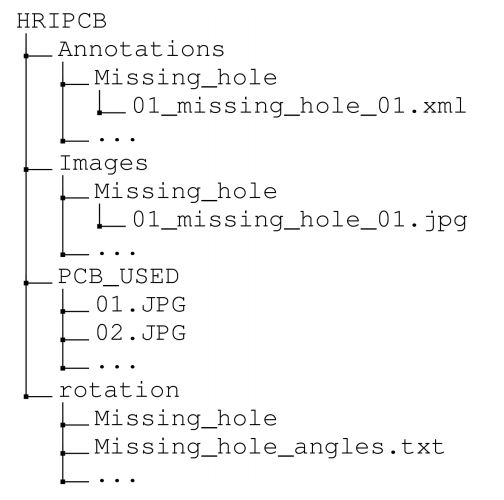
\includegraphics[scale=0.35]{img/img-resultados-hripcb-estrutura.png}
  \label{fig:resultados-hripcb-estrutura}
  \indentedfont[15.2cm]{\citeonline{ref:Huang-et-al}}
\end{figure}


\section{Configuração dos Arquivos para o Treinamento} \label{cap:treinamento-treinamento-config}

Para o treinamento, é necessário que os arquivos do \textit{dataset} escolhido estejam de acordo com o padrão utilizado pela YOLO e as imagens estejam separadas nos subconjuntos de teste e treinamento.

Os arquivos de anotação do \textit{dataset} HRIPC foram convertidos de \textit{.xml} para \textit{.txt} utilizando o textit{script} em Python que está no \autoref{apendice:conversao}.
Esse \textit{script} percorre as pastas de anotação de cada defeito (\autoref{fig:resultados-hripcb-estrutura}), abrindo os arquivos \textit{.xml}, convertendo os dados conforme o padrão necessário para o treinamento e salvando esses dados em um arquivo de texto.

A conversão segue as Equações \ref{eq:resultados-conversao-x} e \ref{eq:resultados-conversao-y} para as coordenadas centrais $x_{center}$ e $y_{center}$ das caixas delimitadoras e as Equações \ref{eq:resultados-conversao-w} e \ref{eq:resultados-conversao-h} para a largura ($width$) e altura ($height$) das caixas delimitadoras, onde os resultados estão normalizados pela largura $x_{img}$ e altura  $y_{img}$ da imagem conforme indicado nos passos do \autoref{apendice:etapas-yolo}.

\begin{equation} \label{eq:resultados-conversao-x}
\mathrm{
  x_{center} = \frac{1}{x_{img}} \cdot ( x_{min} + \frac{x_{max} - x_{min}}{2})
}
\end{equation}

\begin{equation} \label{eq:resultados-conversao-y}
\mathrm{
  y_{center} = \frac{1}{y_{img}} \cdot ( y_{min} + \frac{y_{max} - y_{min}}{2})
}
\end{equation}

\begin{equation} \label{eq:resultados-conversao-w}
\mathrm{
  width = \frac{1}{x_{img}} \cdot (x_{max} - x_{min})
}
\end{equation}

\begin{equation} \label{eq:resultados-conversao-h}
\mathrm{
  height = \frac{1}{y_{img}} \cdot (y_{max} - y_{min})
}
\end{equation}

Além da conversão das coordenadas da caixa delimitadora, é necessário também especificar de maneira numérica qual é o defeito indicado por ela. Os defeitos estão numerados de acordo com a \autoref{tab:resultados-defeitos}.

\begin{table}[!h]
  \begin{center}
  \caption{Representação dos defeitos do conjunto de dados HRIPCB para o treinamento da Rede Neural.}
  \label{tab:resultados-defeitos}
  \begin{tabular}{cc}
    \toprule
    \textbf{Defeito} & \textbf{Representação Numérica}\\
    \midrule \midrule
    Circuito Aberto     & 1 \\
    Curto-Circuito      & 2 \\
    Falta de Cobre      & 3 \\
    Excesso de Cobre    & 4 \\
    Trilha Desconectada & 5 \\
    Falta de Estanho    & 6 \\
    \bottomrule
  \end{tabular}
  \indentedfont[0.96\textwidth]{Elaboração própria (2021)}
  \end{center}
\end{table}

O resultado da conversão do arquivo de anotação em \textit{.xml} do \autoref{apendice:hripcb-xml} está no \autoref{cod:conv}, onde cada linha representa um defeito suas coordenadas seguindo o padrão indicado por \citeonline{ref:Bochkovskiy} no \autoref{apendice:etapas-yolo}.

\lstinputlisting
[caption=Exemplo de arquivo de anotação para treinamento com YOLO.,
label=lst:hripcb,
firstnumber=1,
label=cod:conv]
{cod/anotacoes-HRIPCB.txt}

O \textit{dataset} foi dividido aleatoriamente nos sub-conjuntos treinamento e teste utilizando o \textit{script} do \autoref{apendice:divisao}, com 20\% para testes e o restante para o treinamento.  


O arquivo de configuração \textit{obj.names}

\lstinputlisting
[caption=Arquivo de configuração \textit{obj.data}.,
label=lst:hripcb,
firstnumber=1,
label=cod:obj-data]
{cod/obj.data}

\lstinputlisting
[caption=Arquivo de configuração \textit{obj.names}.,
label=lst:hripcb,
firstnumber=1,
label=cod:obj-names]
{cod/obj.names}


\section{Treinamento} \label{cap:treinamento-treinamento}
O treinamento foi feito no Google Colaboratory, um ambiente que permite a execução de códigos Python em \textit{notebooks} Jupyter, adequado para Aprendizado de Máquina, análise de dados e educação, oferecendo recursos de computação como GPUs de forma gratuita \cite{ref:Colab}.



\subsection{Tranferência de Aprendizado} \label{cap:treinamento-rn}


\section{Resultados} \label{cap:treinamento-resultados}


\chapter{Interface de Aplicação} \label{cap:api}
